\documentclass[11pt]{exam}

\addpoints
\unframedsolutions
%\printanswers

\newcommand{\class}{Math 142}
\newcommand{\term}{Winter 2017}
\newcommand{\examnum}{Midterm 1}
\newcommand{\examdate}{February 3rd, 2017}
\newcommand{\timelimit}{50 minutes}

\setlength{\parindent}{0ex}

\usepackage{microtype}
\usepackage[pdftitle = {Cal Poly Math 351}, pdfauthor = {Tony Mendes}, pdfsubject = {Typesetting}, colorlinks = true, urlcolor = blue, linkcolor = blue, citecolor = blue]{hyperref}

\usepackage{amssymb, amsmath, tikz, mathptmx}

\begin{document}

\begin{coverpages}
\hfill Name:\raisebox{-.5ex}{\rule{.33\textwidth}{.1ex}} 

\bigskip

\begin{center}
\begin{large}
\textbf{\examnum} \\ \textbf{\class, \term} \\ \textbf{\examdate}
\end{large}
\end{center}

\bigskip

\rule{\textwidth}{.1ex}

\bigskip

\begin{itemize}
\item Calculutors are not permitted. 
\item This exam has \numquestions{} questions worth a total of \numpoints{} points.
\item You have \timelimit{} to complete this exam. 
\item These special triangles might be helpful: 
\hfill
\smash{
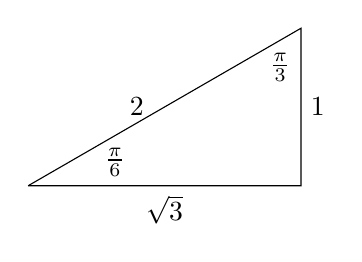
\begin{tikzpicture}[baseline, scale = 2]
\draw (0,0) to node [left = 4] {2} (30:2) to node [right] {1} ++(0,-1) to node [below] {$\sqrt{3}$} (0,0); 
\node at (.55,.15) {$\frac{\pi}{6}$}; 
\node at (1.6,.75) {$\frac{\pi}{3}$}; 
\end{tikzpicture}
\qquad
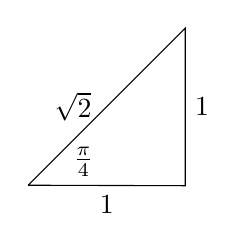
\begin{tikzpicture}[baseline,scale = 2]
\draw (0,0) to node [left = 2] {$\sqrt{2}$} (45:1.41) to node [right] {1} ++(0,-1) to node [below] {1} (0,0); 
\node at (.35,.15) {$\frac{\pi}{4}$};
\end{tikzpicture}
}
\end{itemize}

\bigskip

\begin{center}
\gradetable
\end{center}
\end{coverpages}

\begin{questions}

\question[5]
Evaluate
$\begin{displaystyle}
  \frac{d}{dx} \ln (\sin x)
\end{displaystyle}$.

\begin{solution}[5in]
Using the chain rule, 
\( \begin{displaystyle} 
\frac{d}{dx} \ln (\sin x) = \frac{1}{\sin x} \cos x. 
\end{displaystyle} \) 
\end{solution}

\newpage

\question Let $f(x) =  x^5 + \ln x$ for $x > 0$. 
\begin{parts}
\part[5]
Why does $f(x)$ have an inverse?  

\begin{solution}[4in]
We see that $f'(x) = 5 x^4 + 1/x$ is always positive.  Therefore the function is
always increasing and thus passes the horizontal line test. 
\end{solution}

\part[5]
What is $f^{-1}(1)$? 

\begin{solution}
Since $f(1) = 1$, $f^{-1}(1) = 1$. 
\end{solution}

\end{parts}

\newpage

\question[3] Which of these is a U.S. state?  (Select the single most correct answer): 
\begin{choices}
\choice Confusion
\CorrectChoice California
\choice Mexico
\choice Paranoia
\end{choices}

\question[3] Select all of the true facts about $f(x) = 1/x$.
\begin{checkboxes}
\choice The domain of $f(x)$ is $\mathbb{R}$ 
\CorrectChoice The derivative of $f(x)$ is $-1/x^2$. 
\CorrectChoice The integral of $f(x)$ on $[1,t]$ is $\ln t$.
\end{checkboxes}

\bonusquestion[5] Let $\pi(x)$ be the number of primes less than or equal to $x$. 
Show that 
\[ \left | \pi(x) - \int_2^x \frac{1}{\ln t} \, dt \right| 
\leq \frac{\sqrt{x} \ln x}{8 \pi} \] 
for $x \geq 3000$.  
\end{questions}

\end{document}
